\Problem{Colliding Rocks}{\CollRocks}{
A small rock (mass $m$) is moving to the right on a frictionless table with speed $v$.
}
\ProblemSub{\CollRocksCons}{
It hits a second rock (mass $M$) that is initially at rest on the table. The rocks do not stick together. \\
(i) Is momentum conserved? For what system? \\
(ii) Is energy conserved? For what system?
}
\Solution{\CollRockConsSol}{

Momentum is conserved for the system of both rocks together. There is no net external impulse, as the only forces (those of the collision itself) are internal to the system.

Energy is conserved for this system as well, since a collision without sticking is perfectly elastic, and there is no external work being done (all external forces are perpendicular to the rocks' displacements).
}
\ProblemSub{\CollRocksSpec}{
Our goal is to find the final speed of each rock, but don’t try to solve it yet. \\
Instead, what special cases do you want to think about for this situation? What makes these special cases easier to think about than the general problem?
}
\Solution{\CollRocksSpecSol}{

\noindent\textbf{\underline{Case 1:}} $M \gg m$

If the second rock is very massive, it should basically not budge after being struck by the first rock.

\noindent\textbf{\underline{Case 2:}} $M = m$

If the two rocks are of equal mass, then the first will stop after the collision and the second will be moving at speed $v$. This is exactly like a Newton's cradle desk toy.
}
\Solution{\CollRockCalc}{

\noindent\textbf{\underline{Solution:}}

First, I shall orient myself with a momentum vector diagram. I have assumed that $m$ will still have rightward momentum after the collision, so if I solve for its final speed $v_{m}$ and get a negative number, I know that the rock actually gets turned backward by the collision.
\begin{figure}[h]
	\centering
	\begin{tikzpicture}
		\MVDRows{MVD}
		\MVDCol{mass}{$m$}{MVD}{0.75}
		\MVec{massinit}{0.75}
		\MVec[180]{massdelt}{0.5}
		\MVec{massfin}{0.25}
		\MVDCol{Mass}{$M$}{mass}{0.75}
		\MDot{Massinit}
		\MVec{Massdelt}{0.5}
		\MVec{Massfin}{0.5}
		\MVDCol{sys}{$m$ \& $M$}{Mass}{0.75}
		\MVec{sysinit}{0.75}
		\MDot{sysdelt}
		\MVec{sysfin}{0.75}
	\end{tikzpicture}
\end{figure}

The momentum conservation equation (choosing right as the positive direction) is
\[
mv = mv_{m} + Mv_{M}.
\]
Since the collision is perfectly elastic, we also have conservation of energy:
\[
\frac{1}{2}mv^{2} = \frac{1}{2}mv_{m}^{2} + \frac{1}{2}Mv_{M}^{2}.
\]
We can use these two equations to solve for both unknown final velocities.

First, let us simplify both expressions by dividing through by $m$ (and multiplying the energy equation by 2):
\begin{align*}
	v & = v_{m} + \frac{M}{m}v_{M}, \\
	v^{2} & = v_{m}^{2} + \frac{M}{m}v_{M}^{2}.
\end{align*}
We can write the first equation as $v_{m} = v - \frac{M}{m}v_{M}$ and substitute it into the second to get
\begin{align*}
	v^{2} & = \left(v - \frac{M}{m}v_{M}\right)^{2} + \frac{M}{m}v_{M}^{2} \\
	v^{2} & = v^{2} - 2\frac{M}{m}vv_{M} + \frac{M^{2}}{m^{2}}v_{M}^{2} + \frac{M}{m}v_{M}^{2} \\
	0 & = - 2\frac{M}{m}vv_{M} + \frac{M^{2}}{m^{2}}v_{M}^{2} + \frac{M}{m}v_{M}^{2}.
\end{align*}
Dividing through by $\frac{M}{m}v_{M}$ gives us
\begin{align*}
	0 & = - 2v + \frac{M}{m}v_{M} + v_{M} \\
	\left(1+\frac{M}{m}\right)v_{M} & = 2v \\
	v_{M} & = \frac{2m}{m+M}v.
\end{align*}
Subsituting this into our simplified momentum expression gives us
\begin{align*}
	v_{m} & = v-\frac{M}{m}\frac{2m}{m+M}v \\
	& = \left(1-\frac{2M}{m+M}\right)v \\
	& = \frac{m-M}{m+M}v.
\end{align*}
}
\Solution{\CollRockSense}{
	
\noindent\textbf{\underline{Sensemaking:}}

If $M \gg m$, then $v_{M}$ approaches zero, as predicted. We also see that $v_{m} \approx -v$, so the small rock reflects back at is original speed.

If $M = m$, then $v_{M}=v$ and $v_{m}=0$, which is the Newton's cradle behavior that we predicted.

We didn't talk about $M \ll m$, but it is interesting. In this case, $v_{m} \approx v$ (the more massive object doesn't slow down after the collision) and $v_{M} \approx 2v$ (the stationary object gets launched forward at twice the massive object's speed). In the reference frame of the massive object, the smaller object is leftbound at speed $v$ and reflects to the right at the same speed, much like the previous special case.
}